\section{Introduction}
\begin{quote}
%"If confusion leads to knowledge, then I must be a genius."\begin{flushright}- Larry Leissner\end{flushright}
%     "We often confuse what we wish for with what is." \begin{flushright}- Neil Gaiman \end{flushright}
\end{quote}

Confusion is something that everyone faces in life at some point. 
Whether it is rooted in unclear instructions, 
convoluted rules, or the actions of others, confusion is an 
obstacle that must be overcome to achieve the goals 
we want. How we choose to perceive the world around us has a significant impact in our daily
lives, and unless the choices are very clear (stop or go, on or off, etc.) the potential for confusion 
is always present. This can be a significant problem when we confuse the intent of source code while
developing software. 

Computer science is no stranger to confusing code, and 
sometimes even the intent is to make code inherently 
confusing for security and privacy. Code confusion is when people, whether 
by design or by happenstance, misunderstand the functionality or intent of source 
code. Even misunderstandings of small pieces of the source 
code can lead to larger misunderstandings of the program code as a 
whole. 

Code comprehension is the process by which a developer creates a 
mental model of a software system’s architecture, 
behaviors, and actions based upon the source code. With the increase of more developers on projects, the need
for a uniform understanding of the source between developers is key to the successful development of
software.
As code comprehension is such a vital area for moving forward in 
a software development life-cycle, then it stands to reason that 
making comprehension a more natural process by improving upon the source code is a worthwhile endeavor.

Zokaites describes software as "a 
natural language that must be understood by two separate entities 
for two different purposes"~\cite{zokaites_writing_2002}. One entity is the 
compiler or interpreter that transfers source code into machine 
language, and the other being is developers who need to 
maintain, utilize and create the application. The main difference between programming languages
and natural languages is that
in natural languages 
there is ambiguity that people must interpret. However, programming languages communicate a task to be conducted by a
computer, and thus need to be precise and without any ambiguity.

This does not have an effect on compilers and
interpreters handling confusing code, however problems occur when 
developers are attempting to debug, re-factor, and maintain source 
code. As in the case of \textit{reversed subscript} described by 
Gopstein et al~\cite{gopstein_prevalence_2018}, as shown in Figure~\ref{fig:reversed},
each method individually is seen as producing the same result
from the compiler's view, but the developer often become confused by 
the reversed subscript code snippet on the left. The 
developer can believe that there is a different interpretation when 
the subscript is reversed, rather than when it is not.
These unintentional misinterpretations are what lead 
to code confusion.

\begin{verbbox}[\scriptsize]
void main() {            void main() {
char V1 = 2["qwert"];    char V1 = "qwert"[2];
printf("\%c\n", V1);     printf("\%c\n", V1);
}                        }
\end{verbbox}

\begin{figure}[ht]
\begin{tcolorbox}
\centering
\theverbbox\qquad
\end{tcolorbox}
\caption{Reversed Subscript (left) VS Normal Subscript (right) }
\label{fig:reversed}
\end{figure}



 

%\subsection{Impact of Code Comprehension}\label{sec-impact}
Because software projects and languages are being developed as larger and more complex systems, source code confusion is becoming more
prevalent in a wide array of applications in production. In 
\textit{Code Complete} \cite{mcconnell_code_2004}, McConnell states that industry
averages between 15-50 errors per 1000 lines of delivered code. Therefore, as the number of lines
of code in projects grows so does the amount of errors. By understanding the code thoroughly developers can reduce the potential for errors due to code confusion, which increases the need for better code comprehension methods.

Just during maintenance and re-factoring stages developers spend a major 
portion of their time, approximately 60-90\%~\cite{ward_program_nodate}, on simply trying to understand the
source code. In fact many development teams would
benefit greatly, reducing a significant portion of the 
maintenance and re-factoring overhead by simply making their 
software easier to comprehend.

There are more developers on projects than ever before, and the impact of 
misinterpreting the outcome of code portions can create cascading effects that ripple throughout the project.  With
each module of a program depending on the results of others, a single error can create a ripple effect throughout the entire program.
At implementation time, this can cause a massive overhead in debugging code because the compiler would not 
throw any errors, but the results will be affected all down the line.

Software maintenance is a very costly, broad, and complicated process 
as it requires very deep understanding of the target system source 
code. Moreover, professional
developers must be familiar with the system undergoing change in order to accomplish
the required maintenance tasks \cite{alhindawi_degree_nodate}.

For example, a developer at the financial code supplier IMMUNIO, used a fork to create additional
processes. This developer interpreted an if/then condition incorrectly which was supposed to test for when
the program could stop forking. Since the program continued to fork endlessly, the whole system was taken
down due to the hundreds of connections to the back-end eating up resources. Since the communications were
so bogged down, this meant that their clients were not able to complete transactions quickly enough and
lost millions of dollars \cite{sherman_21_nodate}. 

Also, a similar situation happened in 2012 when the Knight Capital Group needed to replace code that was
years-old but no longer used. Due to a misunderstanding, the flag that was used to call the old code was 
repurposed and sent to the servers without copying over the new code. This "glitch" ended up being
propagated to all the servers when technicians took the code off of the other servers. In 45 minutes the
company sold all the stock it had bought that morning ending in a net loss of 440 million dollars
\cite{sherman_21_nodate}.

With the inter-connectivity of modules in large projects, code comprehension is a major time and cost investment for 
developers. The ability to understand
pre-existing source code is one of the most important elements 
of a continuously successful software
project~\cite{gopstein_understanding_2017}. Take the Linux kernel 
development for example, with hundreds of thousands of lines of 
code and dozens of inter-working modules (as shown in 
 Figure~\ref{fig:kern}), a single confusing bit of 
code can create errors that ripple throughout the entirety of 
the system and would be incredibly hard to track down. 

\begin{figure*}%[htbp]
\centering
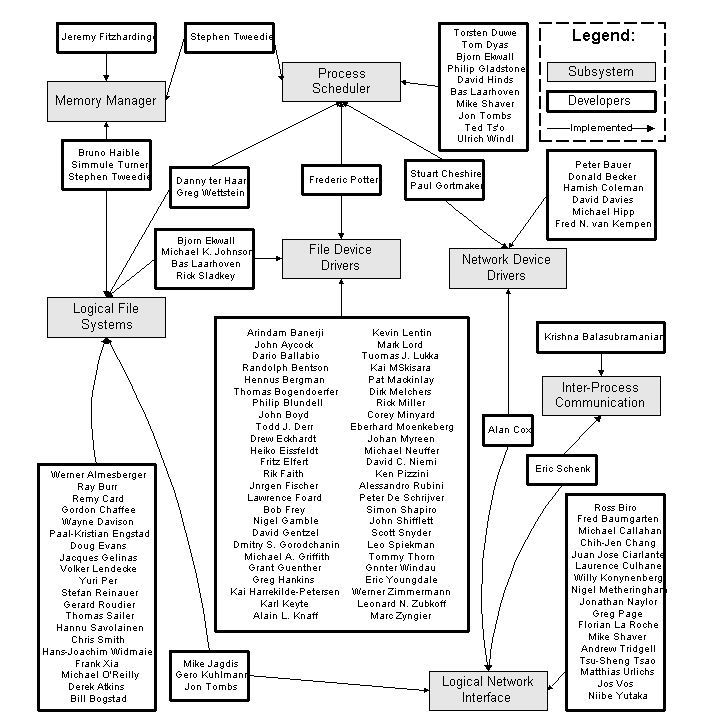
\includegraphics[scale=.75]{images/LinuxKernel}
\caption{Modules of the Linux Kernel and assigned developers \cite{noauthor_conceptual_nodate}}
\label{fig:kern}
\end{figure*}

Code confusion creates an expensive overhead cost to developers 
and is an acknowledged problem in the community 
that has had a number of suggested solutions proposed, but has 
never had a panacea solution. Simply
being able to reliably identify and remove code that can cause 
misunderstandings will enhance productivity and reduce maintenance 
costs~\cite{gopstein_understanding_2017}.

%\subsection{Objective}
This paper will explore the effectiveness of the methods for 
improving code comprehension suggested by the 
measurement of cognitive comprehension in program comprehension 
models, the creation of software clarity metrics to 
increase software readability, the use of coding style guides in 
multi-developer projects, and the inverse relation of
code obfuscation in security. Analysis of the methods that are 
currently available will show that there is still room 
for newer methods of identifying confusing code and the 
combination of current solutions that can greatly increase source 
code comprehension.

%\subsection{Organization}
The following organization method is used to present this research. Section I  
details what code 
comprehension is and why it continues to
be an important field of research. Section~\ref{sec-models} then 
discusses the main three models of code
comprehension, examining their 
common features and differences.  In Section~\ref{sec-current}, 
we will present the
current research methods and tools used to increase code 
comprehension and examine the inversely related field of code obfuscation, and in Section~\ref{sec-compare} we will compare
these methods to determine 
how we can use these principles to affect change towards code 
comprehension. Finally, in Section~\ref{sec-conclude} we will give 
a summary from all the research into code comprehension and where we can go
in future work.